\section{Генерация входных данных}

Для формирования входных данных выделяют два подхода:

\begin{itemize}
	
	\item на основе символьного исполнения, заключающийся в построении системы уравнений на основе условий, которые необходимо выполнить для прохождения конкретного пути в программе;
	
	\item генеративный, заключающийся в применении простых операций вроде инверсии битов или копирования и удаления сегментов данных для формирования новых образцов.
	
\end{itemize}

Далее будут более детально рассмотренны описанные подходы.

\subsection{Символьное исполнение}

Символьное исполнение -- 

\subsection{Генеративный подход}

Генеративный подход, иногда именуемый "умным рандомом", состоит в применении к существующим образцам данных простых операций, в подавляющем большинстве случаев работающих случайным образом, в надежде получить образцы, на которых программа проявит новое поведение. Для применения данного подхода большое значение имеет начальный набор образцов, из которого фаззер может отбирать участки данных.

Не смотря на свою простоту, этот подход зарекомендовал себя как стандарт в индустрии, так как его применение возможно в условиях отсутствия знания о структуре программы или формате данных, ожидаемых ею на входе.

\subsubsection{Генерация при помощи грамматики}

Часто генеративный подход сталкивается с проблемами при работе с программами, вход которых имеет строгую структуру. Например, если мы фаззим интерпретатор языка программирования, подавляющее большинство полученных в результате работы фаззера образцов данных, полученных на основе случайных мутаций, будут отбраковываться модулями лексического и синтаксического анализа, что может привести к неизмеримо большому количеству безуспешных запусков программы. 

Более совершенной разновидностью генеративного подхода, пригодной для работы с структурированными данными, является генерация на основе грамматики. Фаззеру на вход подаются правила, задающие общую структуру данных, а вместо простых операций вроде инверсии битов применяется случайный выбор продукций грамматики, в результате чего получаем синтаксическое дерево. Свернув терминальные узлы синтаксического дерева, получим последовательность байт, которую уже можно подавать на вход программе.

Например, рассмотрим следующую грамматику, описывающую математические выражения:
\begin{align*} % TODO: строки в виде моноширинного текста
	Root &\rightarrow Number \ | \ Root \ Operator \ Root \\
	Number &\rightarrow regex("0|[0-9]\backslash d+") \\
	Operator &\rightarrow "+" \ | \ "-" \ | \ "*" \ | \ "/"	
\end{align*}
где $"+"$ -- терминал, описываемый строкой, а $regex(string)$ -- терминал, соответствующий заданному регулярному выражению. Генерацию ввода по грамматике можно проводить следующим образом рекурсивно: находясь в нетерминале $N$, которому соответствует правило $N \rightarrow E_1 \ | \ ...\  | \ E_n$, случайным образом равновероятно выбрать одно из правил вывода $E_i$, заменить нетерминал $N$ на последовательность терминалов и нетерминалов, и для каждого нетерминала в полученной последовательности операцию повторить. 

При этом нам может потребоваться ввести ограничение на глубину результирующего дерева. В таком случае стоит дополнительно учитывать текущий уровень вложенности, а генерацию дерева ограничить конечным числом попыток. При рассмотрении очередного нетерминала проверим, что оставшийся запас вложенности не нулевой, и в случае, если это не так, посчитаем попытку генерации неудачной и сообщим об этом на уровень выше, попытавшись применить другое правило, а успешной будем считать попытку, в результате которой все нетерминалы в правой части правила вывода были успешно сгенерированы.

После генерации дерева необходимо свернуть его в последовательность байт, которую можно подать программе. Для этого можно также использовать рекурсивный обход, сворачивая поддеревья слева направо, в результате чего мы выпишем все терминалы. Например, для следующего дерева (Рисунок \ref{fig:tree_expansion}) терминалами будут "7", "+", "2", "*", "15", которые свернутся в строку "7+2*15".

\begin{figure}[h]
	\centering
	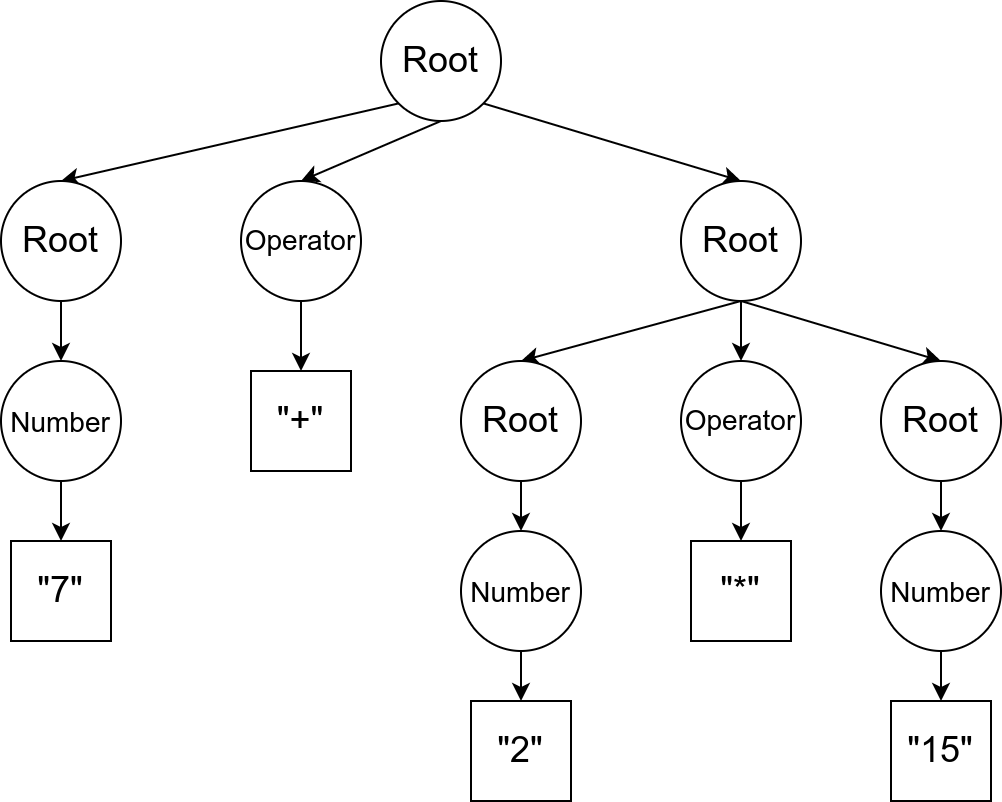
\includegraphics[width=0.5\textwidth]{tree.png}
	\caption{Дерево, построенное по заданной грамматике}
	\label{fig:tree_expansion}
\end{figure}%

При этом возможно сочетание с классическими мутационными алгоритмами за счёт внедрения в результирующее синтаксическое дерево блоков, содержащих двоичные данные.

\subsubsection{Генетические алгоритмы}

% TODO генетические алгоритмы

Примером подобного подхода является iFuzzer, предназначенный специально для фаззинга интерпретаторов языков программирования \cite{ifuzzer}. Данный фаззер руководствуется описанием грамматики целевого языка программирования для генерации тестовых примеров и использует подходы генетических алгоритмов -- fitness function, мутацию и кроссинговер -- для выбора существующих и генерации новых образцов, за счёт чего он способен создавать разнообразные образцы корректных с точки зрения целевого парсера программ. Применение fitness function позволяет ограничить разрастание генерируемых образцов за счёт введения штрафов, зависящих от размера программы, таким образом стремясь к генерации примеров наименьшей длины и наиболее разнообразной популяции.

Также для поддержания семантической корректности при мутации данный фаззер использует подход с переиспользованием литералов, заключающися в ограничении выбора имён переменных из уже существующих в синтаксическом дереве и переименовании переменных при модификации синтаксического дерева в процессе мутации. Это становится возможным благодаря явной разметке в грамматике участков, являющихся именованными сущностями.
